\section{Правила игры}

\subsection{Начало игры}

\subsubsection{Игровой набор}

Для игры используются 136 специальных костей, которые чаще называют \textit{тайлами}. Есть 34 вида тайлов, и каждый из них встречается в наборе ровно четыре раза (34 х 4 = 136). На одной стороне тайла находится значимое изображение, другая же, рубашка, у всех тайлов одинакова.

Тайлы мастей:

\begin{tabular}{ |C{3.5cm}|c|c|c|c|c|c|c|c|c| } 
	\hline
	Масть/номинал & 1 & 2 & 3 & 4 & 5 & 6 & 7 & 8 & 9 \\
	\hline
	Ман \newline & \mahjong{1m} & \mahjong{2m} & \mahjong{3m} & \mahjong{4m} & \mahjong{5m} & \mahjong{6m} & \mahjong{7m} & \mahjong{8m} & \mahjong{9m} \rule[1ex]{0pt}{7ex} \\
	\hline
	Пин \newline & \mahjong{1p} & \mahjong{2p} & \mahjong{3p} & \mahjong{4p} & \mahjong{5p} & \mahjong{6p} & \mahjong{7p} & \mahjong{8p} & \mahjong{9p} \rule[1ex]{0pt}{7ex} \\
	\hline
	Соу \newline & \mahjong{1s} & \mahjong{2s} & \mahjong{3s} & \mahjong{4s} & \mahjong{5s} & \mahjong{6s} & \mahjong{7s} & \mahjong{8s} & \mahjong{9s} \rule[1ex]{0pt}{7ex} \\
	\hline
	Японское чтение & ии & рян & сан & суу & уу & ро & чии & паа & чуу \\
	\hline 
\end{tabular}


Благородные тайлы (обратите внимание, порядок важен):

\begin{tabular}{ |c|C{2cm}|C{2cm}|C{2cm}|C{2cm}| } 
	\hline
	 \rule[0ex]{0pt}{7ex} Ветра & \mahjong{1z} \newline Восток & \mahjong{2z} \newline Юг & \mahjong{3z} \newline Запад & {\mahjong{4z} \newline Север} \\
	\hline
	Японское чтение & тон & нан & ся & пей \\
	\hline
\end{tabular}

\begin{tabular}{ |c|C{2cm}|C{2cm}|C{2cm}| } 
	\hline
	 \rule[0ex]{0pt}{7ex} Драконы & \mahjong{5z} \newline Белый & \mahjong{6z} \newline Зеленый & \mahjong{7z} \newline Красный \\
	\hline
	Японское чтение & хаку & хацу & чун \\
	\hline
\end{tabular}

Для подсчета очков в игре используются палочки следующих номиналов:

\begin{tabular}{ |c|c|c| } 
	\hline
	
\includegraphics{tenbo10000} & 10000 очков & x1 \\
	
\includegraphics{tenbo5000} & 5000 очков & x2 \\
	
\includegraphics{tenbo1000} & 1000 очков & x9 \\
	
\includegraphics{tenbo100} & 100 очков & x10 \\
	\hline
\end{tabular}

Иногда можно встретить в наборах палочки номиналом 500 очков, как правило они выглядят так же как палочки на 100 очков, но окрашенные в зеленый цвет.

Общее количество очков в начале игры у каждого игрока равно 30000. Количество палочек в наборе может также отличаться, например может быть три палочки по 5000 и четыре по 1000, главное чтобы общее количество соответствовало указанному.

Также в игре используются:
\begin{itemize}
	\item Индикатор первого дилера - небольшая пластинка с изображением восточного ветра (\textnihon{東}) с одной стороны и южного ветра (\textnihon{南}) с другой;
	\item Два шестигранных кубика с цифрами от 1 до 6.
\end{itemize}

\subsubsection{Подготовка к игре}

В риичи-маджонг играют вчетвером. Для игры используют небольшой квадратный стол (~75х75 см), с каждой стороны которого садится по игроку. Каждому месту за столом присваивается условная сторона света, и расположены они в порядке тайлов ветров против часовой стрелки: восток (\textnihon{東}), юг (\textnihon{南}), запад (\textnihon{西}), север (\textnihon{北}), т. е. порядок «неправильный» и отличается от настоящего расположения сторон на карте мира\footnote{Порядок ветров соответствует расположению сторон света на карте звездного неба.}. Выбор мест производится по договорённости или по жребию. Способ распределения мест таков: на стол кладутся четыре разных тайла ветров рубашкой вверх, игроки вытягивают их по очереди, и каждый занимает соответствующее место. Ветер, соответствующий месту игрока, называется \textit{ветром места}. 

Игрок, вытянувший восток, занимает в игре особое положение \textit{дилера}. Рядом с ним в начале игры кладётся индикатор первого дилера. Обычно дилер выбирает место за столом, остальные рассаживаются относительно него согласно вытянутым ветрам.

Игра делится на раунды, также названные по сторонам света – восточный (первый) и южный (второй), и раздачи. Существует два варианта партий: короткая игра, где играется только восточный раунд, называется \textit{тонпусен}, длинная и с восточным, и с южным – \textit{ханчан}. Ветер, соответствующий текущему раунду, называется \textit{ветром раунда}. Раунд по умолчанию состоит из четырёх раздач (хотя в отдельных случаях, оговорённых правилами, могут назначаться дополнительные раздачи), и каждую новую раздачу происходит сдвиг сторон света за столом на одно место против часовой стрелки: игрок, в первой раздаче бывший на юге, во второй оказывается дилером, в третьей – севером и т. д, сами игроки при этом не пересаживаются. Таким образом, смена раунда происходит, когда дилерство возвращается к игроку, бывшему дилером в первой раздаче. Индикатор первого дилера всё время остаётся лежать рядом с дилером первой раздачи; во время восточного раунда он повёрнут вверх стороной, где нарисован иероглиф востока, а с началом южного переворачивается. Для указания на дилера текущей раздачи с его стороны стола после подготовки к раздаче кладутся кубики.

Перед началом каждой раздачи игроки кладут все тайлы на стол рубашкой вверх и тщательно их перемешивают. После этого каждый игрок строит перед собой «стену» высотой в 2, шириной в 1 и длиной в 17 тайлов рубашкой вверх, размещая её так, чтобы в итоге четыре участка стены от разных игроков образовали замкнутый квадрат. Затем дилер бросает кубики и отсчитывает против часовой стрелки столько сторон квадрата, сколько выпало на кубиках суммарно, начиная со своей стороны (на рис.1 показан пример для выпавшей суммы 8).

\begin{figure}[H]
	\centering
	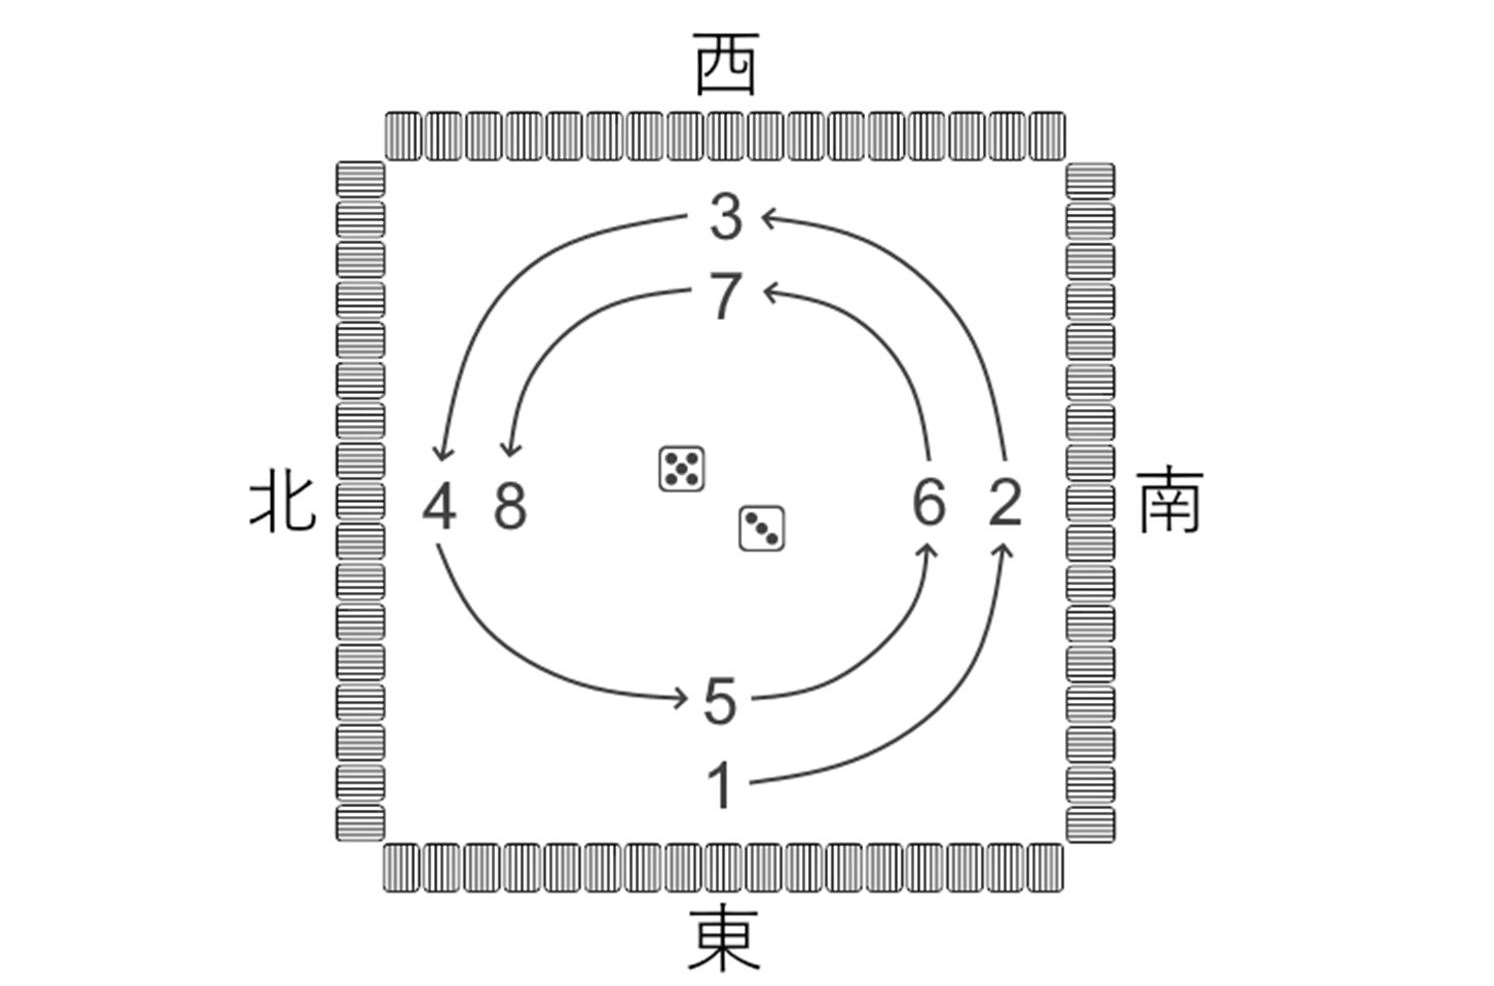
\includegraphics[width=16cm]{table-deal-start.png}
	\caption{Определение разлома стены}
\end{figure}

Затем игрок, на чью сторону указал дилер (в примере выше – север) отсчитывает от правого конца своей стороны стены столько тайлов, какое число выпало на кубиках до этого (в примере – 8) и немного отодвигает их от соседних тайлов вправо, создавая разлом стены. После этого он отсчитывает от разлома в обратную сторону 7 тайлов и делает второй разлом, обособляя получившуюся группу из 14 тайлов (см. рис.2). Эта группа называется мёртвой стеной и не разбирается в процессе игры. Оставшаяся часть стены называется живой стеной и используется во время раздачи для получения игроками тайлов (наподобие колоды карт). Разбирается она стопками верхний-нижний по часовой стрелке, начиная с верхнего тайла первой стопки после разлома и заканчивая нижним последней перед мёртвой стеной. Стена считается непрерывной, и переход через углы не имеет никакого значения как при формировании мёртвой стены, так и при последующем разборе.

Третий верхний тайл от конца мёртвой стены переворачивается рубашкой вниз (на рисунке это 6 ман) и служит в данной раздаче индикатором доры – тайла, дающего дополнительные очки при его наличии в руке. Подробно о дорах и принципе работы индикаторов рассказано в разделе VIII.

\begin{figure}[H]
	\centering
	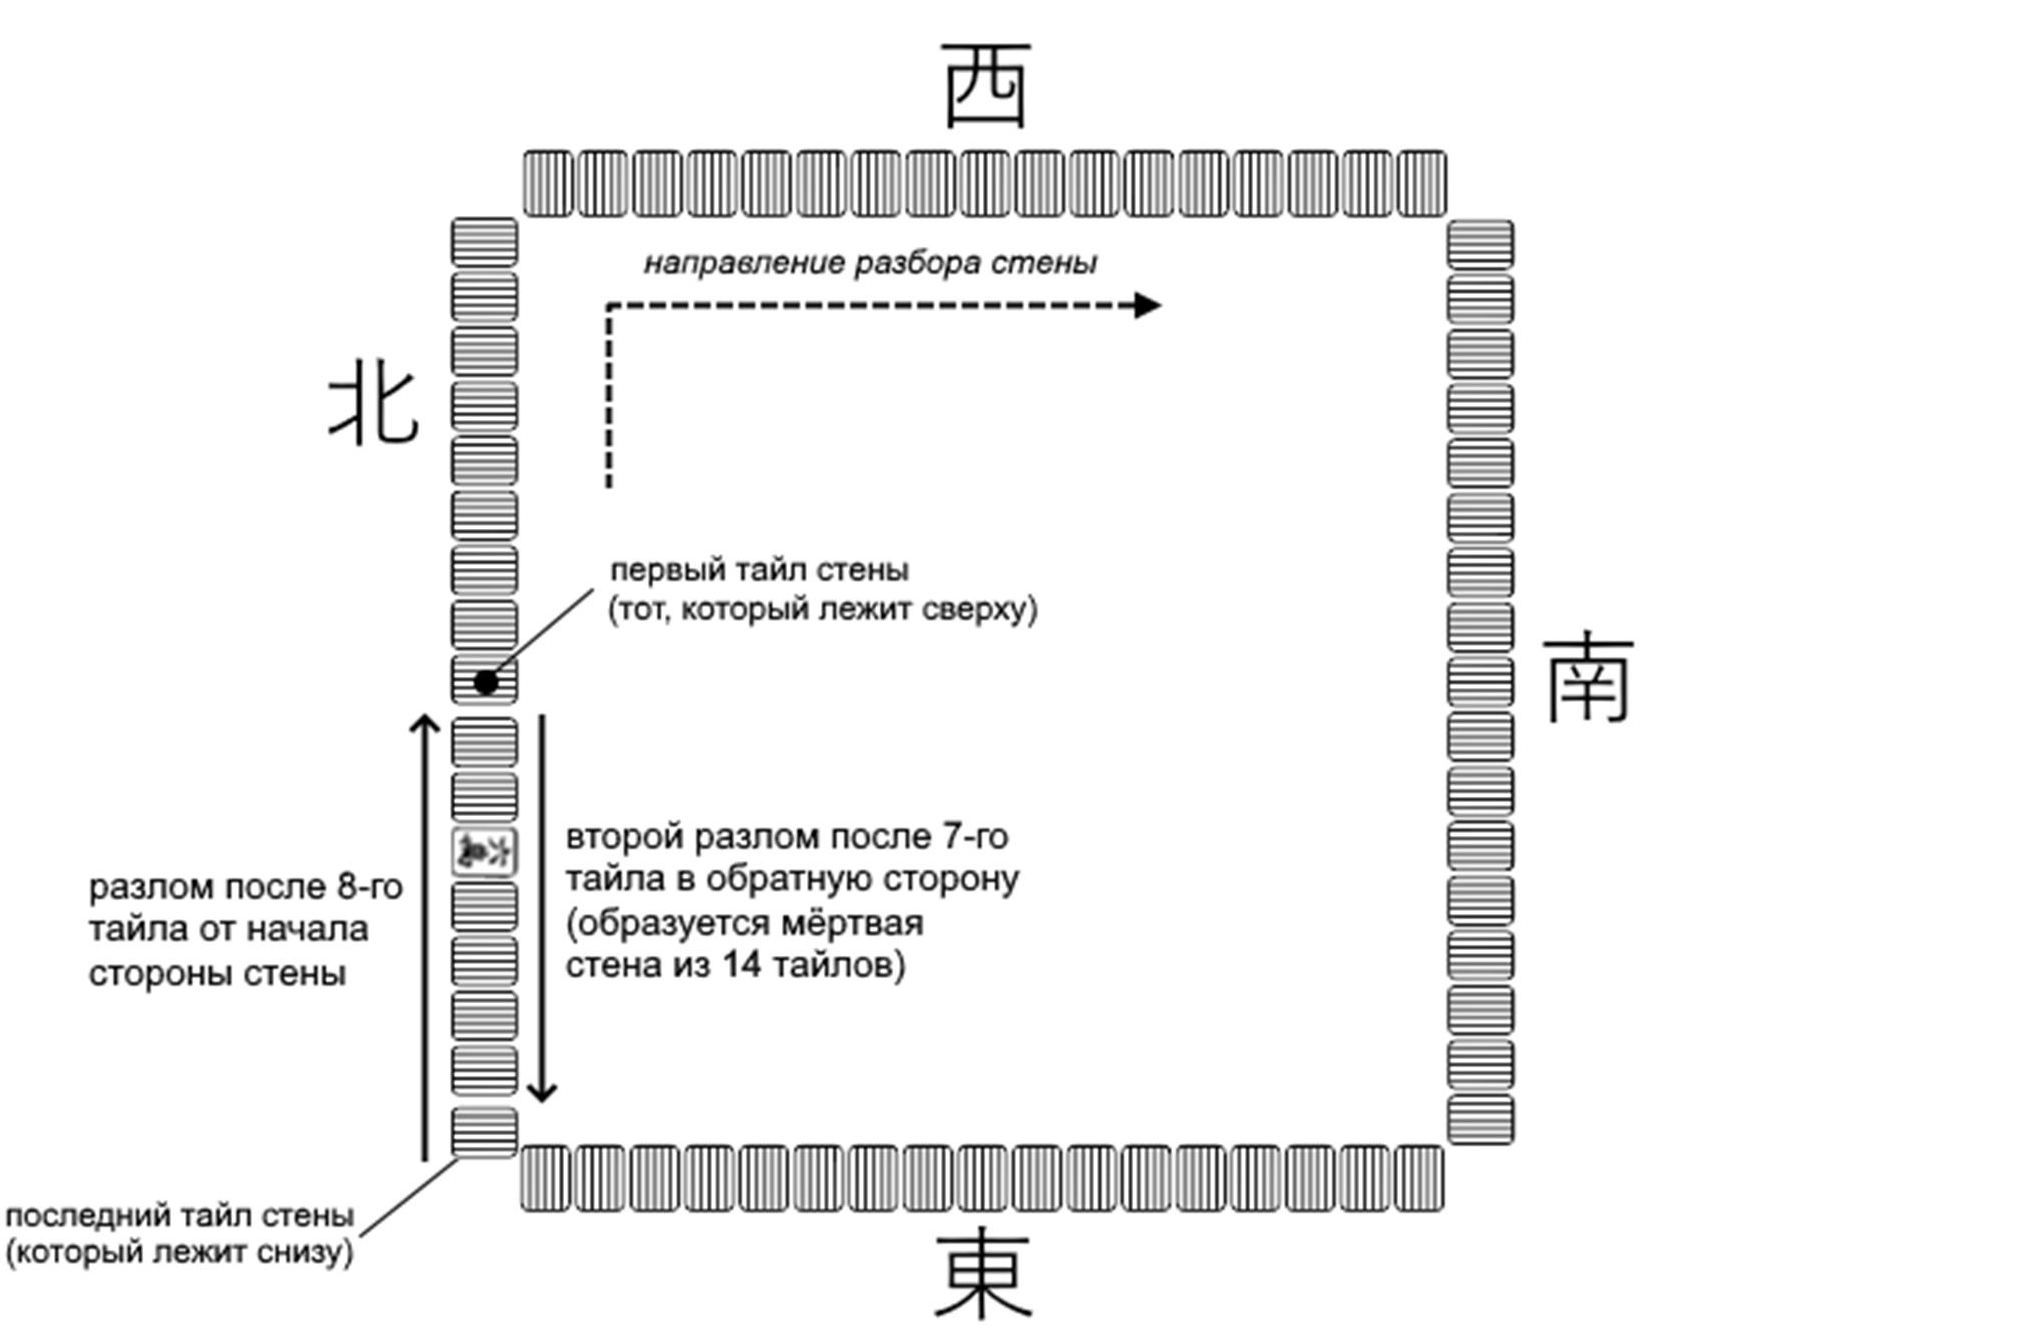
\includegraphics[width=16cm]{table-deal-start-2.png}
	\caption{Мертвая и живая стены}
\end{figure}

После открытия индикатора доры игроки берут себе со стены тайлы в стартовые руки. Начиная с дилера по очереди против часовой стрелки игроки начинают брать от начала живой стены по четыре тайла (две стопки по 2), пока у каждого не окажется 12 тайлов. После этого игроки в том же порядке берут ещё по одному тайлу (порядок разбора – всегда от верхнего к нижнему), а затем дилер берёт себе ещё один тайл (см. рис.3). Таким образом, в начале раздачи дилер имеет 14 тайлов, а остальные – по 13. Тайлы своих рук игроки расставляют перед собой в ряд вертикально изображением к себе, так, чтобы остальные видели только их рубашки. Для удобства игроки сортируют руки: ставят рядом тайлы одной масти по порядку номеров и одинаковые благородные тайлы. Допустим, игрок взял себе в стартовую руку следующие тайлы:

\mahjong{5m 6s 4m 8s 3z 9m 7z 2z 1s 3m 7z 7s 4m}

Он может отсортировать их следующим образом:

\mahjong{1s 678s 34459m 2377z}

Разные масти могут быть отсортированы слева направо или справа налево, а разные благородные тайлы могут стоять в разных местах – всё зависит от удобства для игрока и времени, затрачиваемого на сортировку. В данном описании правил в дальнейшем для простоты все руки будут показаны отсортированными одинаково: ман, пин, соу слева направо, ветра по порядку, драконы по порядку.

В компьютерном маджонге построение стены, её разлом, набор и сортировка стартовых рук как правило происходят автоматически, и когда начинается раздача игроки сразу же видят свои отсортированные стартовые руки и индикатор доры. 

\begin{figure}[H]
	\centering
	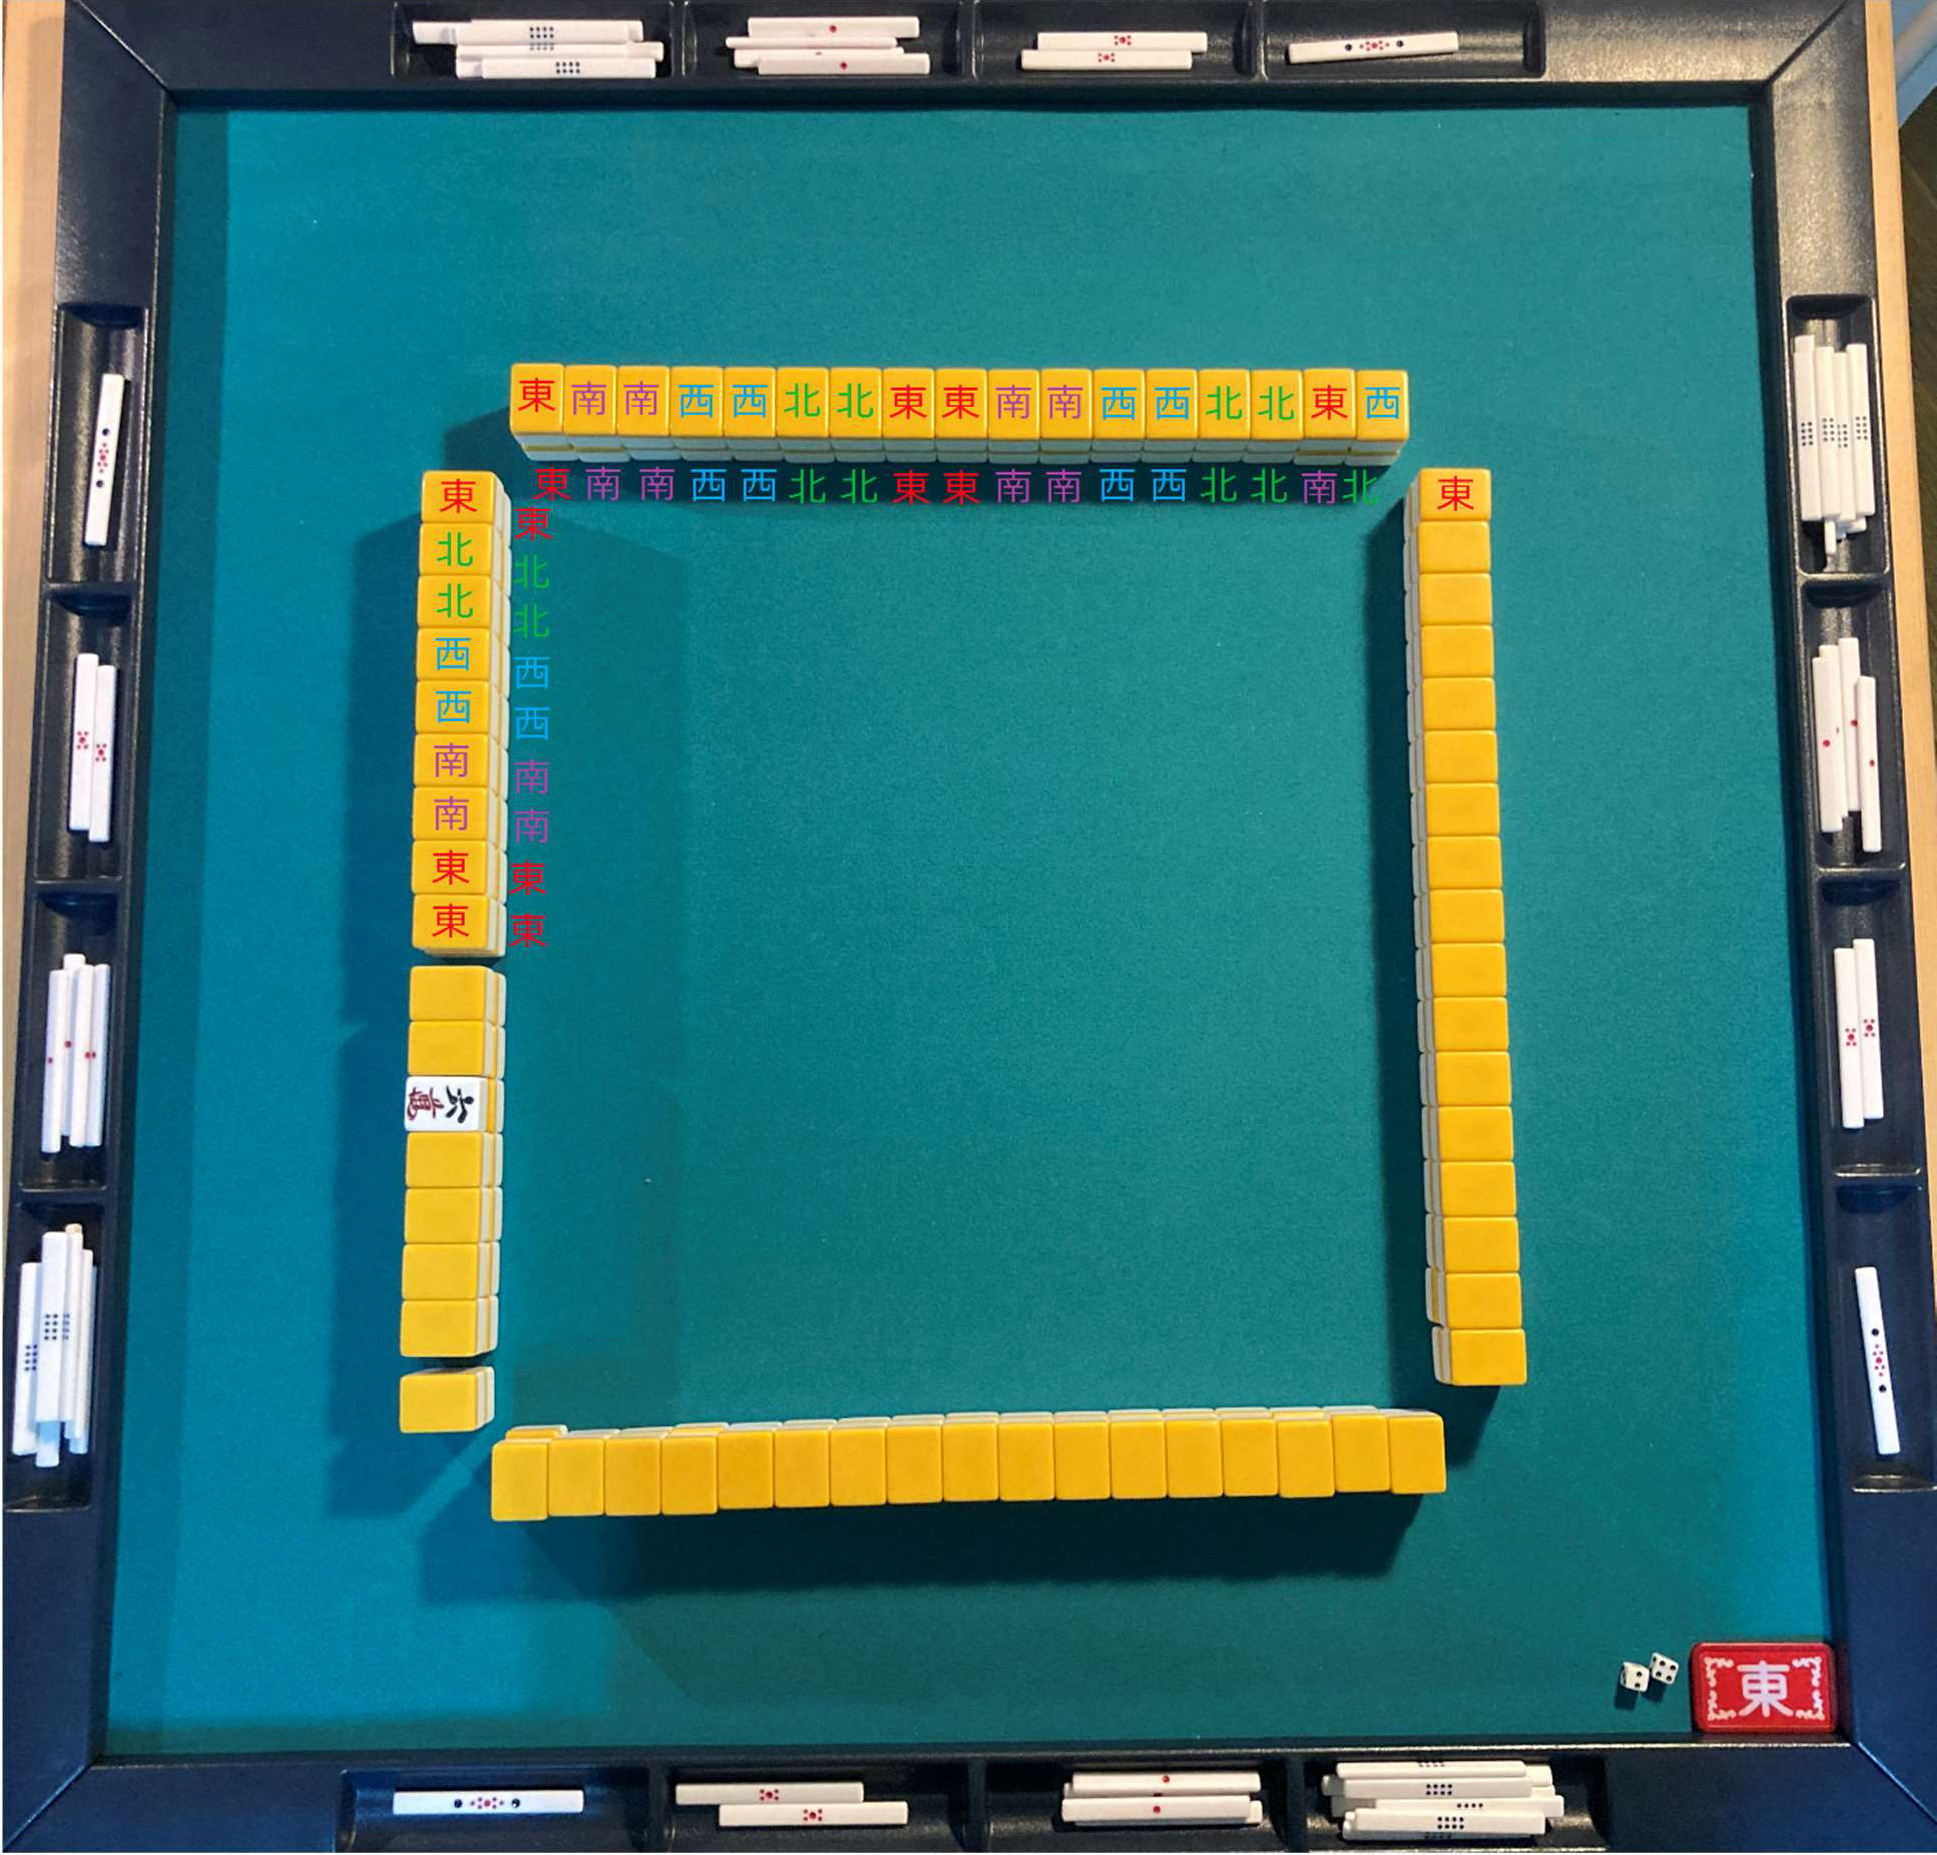
\includegraphics[width=16cm]{table-deal-start-3.png}
	\caption{Порядок разбора стены, фото}
\end{figure}

Обратите внимание на подписи тайлов - они показывают, какой игрок должен их взять (верхние тайлы стены подписаны прямо на рубашке, нижние – рядом). Предположим, что сейчас идёт первая раздача восточного раунда: индикатор первого дилера повёрнут иероглифом востока кверху, а кубики как индикатор текущего дилера лежат рядом с ним, т. е. первый дилер является дилером в этой раздаче.

\subsection{Ход раздачи}

В ходе раздачи, которая начинается сразу же после набора и сортировки всеми стартовых рук, игроки изменяют состав своих рук, набирая в них по одному новые тайлы с живой стены и выбрасывая ненужные. Цель каждого игрока в раздаче – собрать в руке четыре сета и одну пару (два одинаковых тайла). При объявлении кем-либо победы с готовой рукой раздача заканчивается. Цель всей игры – набрать как можно больше очков, получаемых в основном за собранные руки.

Сет – это определённая комбинация из трёх или четырёх тайлов. Они бывают трёх видов:
\begin{itemize}
	\item Три одинаковых тайла - \textit{пон};
	\item Четыре одинаковых тайла – \textit{кан};
	\item Последовательность из трёх тайлов одной масти подряд (по типу 1-2-3, 3-4-5 и т. п.) – \textit{чи}. Последовательности можно собирать только из тайлов мастей, и в них не должно быть перехода через девятку: 8-9-1 и 9-1-2 не засчитываются как чи.
\end{itemize}

Один тайл не может одновременно входить в два сета. В примере ниже в руке уже есть готовый пон из 4 ман, чи 7-8-9 ман и пара красных драконов, но последовательность 3-4-5-6-7 пин не засчитывается за два чи: для завершения этой формы в два сета требуется получить ещё один тайл (2, 5 либо 8 пин).

\mahjong{444789m 34567p 77z}

В руке из примера выше 13 тайлов, как и в любой руке не-дилера в начале раздачи, но выигрышная рука должна содержать как минимум 14 тайлов (3+3+3+3+2, если же в руке есть каны, число тайлов может доходить до 18). Четырнадцатый тайл игроки получают в свои ходы во время раздачи: раздача начинается с хода дилера, который сбрасывает из руки один из своих 14 тайлов, кладя его рубашкой вниз в центр стола; затем ход переходит к следующему игроку против часовой стрелки, который берёт первый тайл из оставшейся части живой стены и также сбрасывает один тайл из своей руки (можно сбрасывать и тайл, только что взятый со стены – такой сброс называется \textit{цумогири}). Затем ход переходит к следующему игроку, и так раздача продолжается до тех пор, пока кто-либо не соберёт руку и объявит победу, или же пока в живой стене не закончатся тайлы. 

Ходы в риичи-маджонге обязательны, пропускать взятие со стены либо сброс нельзя. Каны, а вместе с ними и руки, содержащие более 14 тайлов, возможно образовать специальными объявлениями, о которых рассказывается в следующем разделе. Ходы четырёх игроков, начиная от дилера, образуют круг раздачи. После окончания круга ход вновь переходит к дилеру, и начинается следующий круг. Группы сброшенных тайлов в центре стола называются сбросами или \textit{дискардами}. Каждый игрок имеет свой отдельный дискард. Тайлы следует выкладывать в сброс слева направо тремя рядами по 6 штук (начиная с ближнего к центру стола и далее по направлению к себе); четвёртый же ряд чаще не начинают, а вместо этого продолжают третий.

\begin{figure}[H]
	\centering
	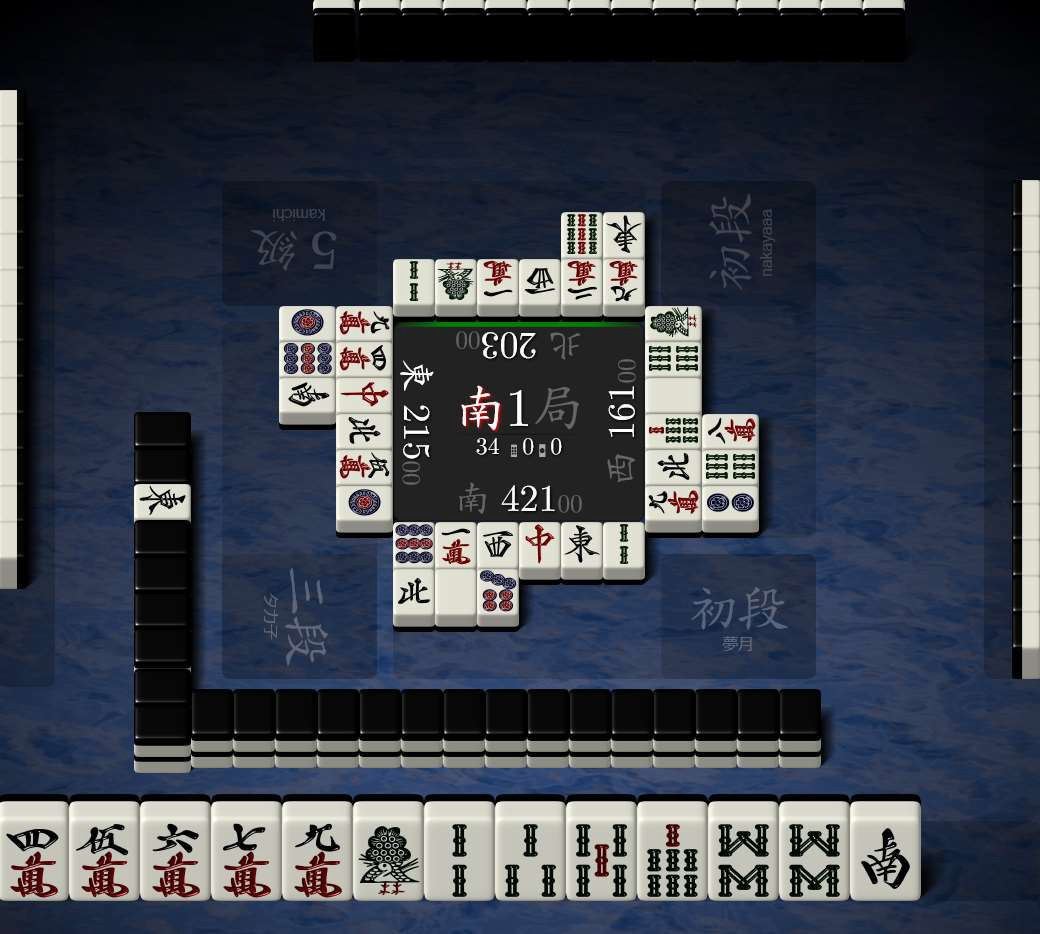
\includegraphics[width=16cm]{tenhou-deal.jpg}
	\caption{Пример раздачи на сервере tenhou.net}
\end{figure}

Рассмотрим вид стола в процессе раздачи на онлайн-сервере tenhou.net (рис.4). В центре – указатель раунда и номера раздачи за раунд (южный, первая) и указатели мест игроков со счётчиками очков (мы юг с 42100 очков; на онлайн-серверах вместо палочек используются цифровые счётчики). Вокруг центра – дискарды игроков, ниже – живая стена, слева – мёртвая стена с индикатором доры восточным ветром. По краям стола расположены руки игроков. Сейчас 9-й круг, ход севера: он получил тайл со стены, но ещё не совершил сброс. Пришедший со стены тайл сначала ставят отдельно (здесь он стоит слева от основной руки, если смотреть от нас), и встраивают в руку только после сброса, если сброшен другой тайл.

\subsection{Объявления в игре}

% TODO: Сорокин

\subsection{Фуритен и временный фуритен}

Правило \textit{фуритен} (\textnihon{フリテン}), или правило упущенного сброса, запрещает игроку объявлять рон, если хоть один из выигрышных тайлов, завершающих руку, лежит у него в дискарде. При этом как дискард учитываются и тайлы, взятые оттуда для сетов другими игроками. Именно из-за этого при объявлениях сетов требуется указывать какой тайл был взят и с кого из противников, кладя один из тайлов боком с соответствующей стороны.

Например, рассмотрим игрока со следующей рукой:

\mahjong{33456678m 23p 678s}

Предположим, дискард у игрока следующий:

\mahjong{1p 4z 7z 2s 4s 9m}

В данном случае игрок не может объявить рон ни при сбросе противником 1 пин, ни при сбросе 4 пин, потому что в его дискарде есть «упущенный» выигрышный тайл 1 пин. При этом ограничений на объявление цумо нет. Если игрок перестроит свою руку так, чтобы сброшенные в дискард тайлы не завершали выигрышное ожидание, фуритен перестанет действовать, и он снова сможет объявлять рон. Например, это будет возможно если руку выше изменить следующим образом взятием 5 пин и сбросом 2 пин: 

\mahjong{33456678m 35p 678s}

В этом случае ожидание на 1 пин пропадёт, и игрок сможет объявить рон на сброшенную кем-либо 4 пин. 

Фуритен даёт возможность для игры в защиту: тайлы, лежащие в сбросе у противника, можно уверенно сбрасывать, не опасаясь, что он объявит на них рон (при победе по рону игрок получает очки за счёт сбросившего выигрышный тайл; о выплатах см. раздел IX). Есть и более продвинутые приёмы защиты, основанные на фуритене, которым посвящены отдельные специализированные статьи, в данном руководстве не рассматриваемые.

\textit{Временный фуритен} – это отдельное правило, которое не позволяет игроку объявлять рон, если на текущем круге считая от хода игрока уже был сброшен какой-либо из выигрышных для него тайлов. Действие временного фуритена заканчивается с первым же ходом игрока – в момент, когда игрок формально может сменить ожидание. Допустим у нас на нашем ходу имеется следующая рука:

\mahjong{123456789m 99s 11z}

В случае если игрок справа сбросил 9 со и мы пропустили возможный рон, а сразу за ним игрок напротив сбрасывает восток или ещё одну 9 со, объявлять рон на этот тайл нельзя, потому что на этом круге рон уже был пропущен. Если же кто-то ещё раз сбросит 9 со или восток уже после следующего нашего хода, рон объявить будет можно.

Временный фуритен существует для предотвращения избирательности в объявлении рона, но иногда действует во вред игрокам в темпае, если после одного пропущенного выигрышного тайла на том же круге сбрасывается тайл, дающий руке большую стоимость, чем первый. Если игрок пропустил один рон после объявления риичи, из-за временного фуритена он не может победить по рону до конца раздачи, т. к. после риичи сменить ожидание невозможно (подробно о риичи рассказывается в посвящённом ему разделе VII).

\subsection{Яку: условия победы}

Для объявления победы необходимы не только четыре сета и пара в руке, но и выполнение хотя бы одного \textit{яку} – условия победы, приносящего руке стоимость. Рука без яку не имеет стоимости, и \textunderscore{с такой рукой объявлять победу нельзя}, даже если собраны все сеты и пара. Яку бывают двух типов: это либо наличие определённых комбинаций тайлов в руке, либо особые игровые ситуации, при которых происходит победа. Стоимость яку измерима: каждое из них имеет фиксированную стоимость в \textit{ханах} (яп. \textnihon{飜} или \textnihon{翻}) – специальных единицах, используемых для удобства, которые при подсчёте общей стоимости руки переводятся в очки.

\subsubsection{Комбинационные яку}

Таких яку довольно много: общепринятыми считаются 28 комбинаций. Полный список комбинаций, действительных для текущих правил, приведен в приложении. Рассмотрим некоторые самые часто встречающиеся яку.

\textbf{Тан'яо}\footnote{Читается как "танъяо", апостроф здесь и далее обозначает границу между отдельными слогами в японском чтении.}: все тайлы в руке – средние. Средние тайлы – это тайлы мастей номиналом с 2 по 8. Если рука состоит только из таких тайлов, она содержит яку тан'яо, и с такой рукой в темпае при получении выигрышного тайла можно объявлять победу. Тан'яо стоит 1 хан: соответственно, столько же будет стоить и рука. Это яку действует и на открытой, и на закрытой руке\footnote{Некоторые яку не действуют на открытой руке вообще. Существуют также яку, стоимость которых на открытой руке будет ниже, чем на закрытой.}. Пример выигрышной руки:

\mahjong{333678p 2234s}\hfill \mahjong{5'67s}

Выигрышные тайлы: \mahjong{25s}

Существует и яку-противоположность тан'яо – \textbf{хонрото}, рука, состоящая только из крайних и благородных тайлов. Таких тайлов меньше, и собирать сеты из них сложнее, и поэтому хонрото стоит больше – 2 хан. Стоимость яку зависит от сложности их сбора, и поэтому одна из главных задач игрока во время раздачи – оптимальный выбор между дорогими рискованными и простыми в сборе, но дешёвыми яку. Пример:

\mahjong{111m 99p 999s 11122z}

Выигрышные тайлы: \mahjong{9p2z}

\textbf{Чанта}: каждый сет и пара содержит хотя бы один крайний или благородный тайл. Более лёгкий вариант яку на крайних и благородных тайлах, чем хонрото. Стоимость чанты зависит от закрытости руки: в закрытой руке она стоит 2 хан, в открытой – 1. На открытой руке чанта стоит 1 хан, на закрытой - 2 хан. Пример:

\mahjong{11123m 789p 13s 333z} 

Выигрышные тайлы: \mahjong{2s}

\textbf{Тойтой}: все сеты – поны или каны. Тойтой в любой руке стоит 2 хан. Пример:

\mahjong{44499m44z}\hfill \mahjong{8'88m 11'1s}

Выигрышные тайлы: \mahjong{9m4z}

Яку можно сочетать друг с другом – в таких случаях стоимости всех яку в руке суммируются (за некоторыми исключениями; все исключения описаны в приложении). Например, в руке с тойтоем только на средних тайлах также есть тан'яо, и поэтому она стоит 3 хан. Хонрото – это одновременно и тойтой (если только это не особая рука читойцу; о ней см. ниже), потому что чи из одних крайних и благородных тайлов собрать нельзя, и из-за этого такая рука стоит минимум 4 хан суммарно за оба яку. Это объясняет, почему редкое и сложное в сборе хонрото так несильно отличается по стоимости от куда более простых тан'яо и чанты.

Некоторые яку невозможно сочетать, потому что их условия противоречат друг другу. Например, чанта не сочетается с тан'яо, потому что требует наличия крайних или благородных тайлов, которых в руке с тан'яо быть не может. В других случаях теоретически возможные сочетания яку запрещены правилами. В принципе, рука с хонрото всегда одновременно содержит в себе и чанту – ведь сеты полностью из крайних или благородных тайлов всегда содержат один такой тайл, то есть условие для чанты более, чем выполнено. Но это сочетание запрещено правилами, и поэтому такая рука будет стоить только 4 хан, а не 5 или 6, как было бы с надбавкой за чанту. В основном запрещены сочетания именно таких похожих яку-«апгрейдов».

Противоположность есть и у тойтоя: это \textbf{пинфу}, яку из одних последовательностей. Стоит пинфу 1 хан. Однако просто собрать руку из одних чи и пары очень легко, и для получения пинфу нужно соблюсти несколько дополнительных условий:
\begin{itemize}
	\item Рука должна быть закрытой;
	\item Пара в руке не должна состоять из драконов, ветров раунда или ветров места;
	\item Ожидание в темпае должно быть в две стороны, т.е. последний незавершённый сет должен состоять из двух средних тайлов подряд (например, форме 7-8 для завершения чи подходит тайл с любой стороны: 6 или 9; такое ожидание называется \textit{рянмен}). Ждать в темпае пару уже со всеми завершёнными чи тоже нельзя.
\end{itemize}
Пример руки с пинфу:

\mahjong{233445m 23p 789s 22z}

Выигрышные тайлы: \mahjong{14p}

Обратите внимание, что эта рука содержит пинфу только если идёт не южный раунд и собравший её игрок сидит не на юге, иначе южный ветер будет ветром раунда или места. Рассмотрим другую очень похожую руку:

\mahjong{233445m 12p 789s 22z}

Эта рука не содержит пинфу из-за неправильной формы выигрышного ожидания: не в две стороны, а лишь в одну, поскольку форма 1-2 закрывается только тройкой. Это рука без яку-комбинаций.

Именно из-за требований некоторых яку к ожиданию в темпае игрокам запрещается встраивать выигрышный тайл в руку – иначе другие игроки после открытия руки не смогут его проверить. 

Требования некоторых яку относятся не ко всей руке, а только к отдельным сетам. Примером такого яку служит \textit{якухай}: пон или кан любых драконов, ветров раунда или ветров места. Якухай стоит 1 хан, засчитывается и в открытой, и в закрытой руке. Если в руке несколько сетов драконов или нужных ветров, может удваиваться, утраиваться и т. д. Когда ветер раунда является одновременно ветром места, наличие сета из такого ветра даёт 2 хан – это двойной якухай.

\mahjong{56799m 234s 77z}\hfill \mahjong{11'1z}

Выигрышные тайлы: \mahjong{9m7z}

Эта рука будет иметь разную стоимость в зависимости от игрока и раунда, в который она была собрана. Если её собрал дилер в восточный раунд, она будет стоить 3 хан: 2 за двойной якухай (восточные ветра) плюс 1 за обычный (красные драконы). Для дилера в другой раунд она будет стоить только 2 хан: по 1 хан за каждый сет. Для не-дилера в восточный раунд она также будет стоить 2 хан - по одному за сеты драконов и ветров раунда, а в южный – только 1 хан за сет драконов, потому что восток не будет ни ветром раунда, ни ветром места.

Якухай стоит немного, но занимает только один сет, и поэтому хорошо сочетается со многими другими яку и часто используется в дополнение к ним для повышения стоимости рук: например, нередко встречаются сочетания якухая с тойтоем или чантой.

\textit{Иццу}: три чи 1-2-3, 4-5-6 и 7-8-9 в одной масти (образующие последовательность от 1 до 9).

\mahjong{12223456789p 11s}

Выигрышные тайлы: \mahjong{2p1s}

Иццу стоит 1 хан в открытой руке и 2 хан в закрытой.

\textit{Иипейко}: два полностью одинаковых чи в закрытой руке. Стоит 1 хан, в открытой руке не засчитывается. В руке ниже – сочетание иипейко и пинфу, т. е. она стоит 2 хан. Сеты в бамбуках также завершает 1 соу (1-2-3, 2-3-4), но тогда двух одинаковых сетов не получится, и рука будет стоить только 1 хан за пинфу.

\mahjong{333m 78999p 22334s}

Выигрышные тайлы: \mahjong{14s}

\textit{Саншоку доджун}, или просто \textit{саншоку}: одинаковые по номиналу чи в трёх мастях. Стоит 1 хан в открытой руке и 2 хан в закрытой. В руке ниже – сочетание с пинфу и тан'яо, рука стоит 4 хан.

\mahjong{23466m 234p 23445s}

Выигрышные тайлы: \mahjong{36s}

\textit{Чиитойцу} – это одно из двух яку-исключений, позволяющих выиграть без четырёх сетов. Для получения этого яку нужно собрать в руке 7 пар (четыре одинаковых тайла не считаются за две пары):

\mahjong{7799m11233p88s55z}

Выигрышные тайлы: \mahjong{2p}

Чиитойцу стоит 2 хан, и собрать его возможно только в закрытую, потому что делать объявления пар нельзя. Оно не сочетается с иипейко, так как пары не могут одновременно считаться за чи, и поэтому рука-пример стоит 2 хан, а не 3. Однако некоторые яку, не требующие наличия сетов, например, тан’яо или хонрото, можно собрать и в виде семи пар в сочетании с чиитойцу.

\textit{Хон'ицу} – это рука, состоящая только из тайлов одной масти и любых благородных тайлов:

\mahjong{34455668p 33z} \hfill \mahjong{66'6z}

Выигрышные тайлы: \mahjong{7p}

Стоит 2 хан в открытой руке и 3 в закрытой. В примере сочетание открытого хон'ицу (2 хан) и якухая (1 хан) – рука стоит 3 хан. 

\textit{Чин'ицу} – это рука полностью из тайлов одной масти.

\mahjong{1222345667788s}

Выигрышные тайлы: \mahjong{69s}

Это дорогое яку стоит 5 хан в открытой руке и 6 в закрытой. В примере рука содержит закрытое чин'ицу (6 хан), пинфу (1 хан) и закрытое иццу (2 хан), и стоит суммарно 9 хан. Сеты в ней интерпретируются следующим образом:

\noindent\mahjong{123s-456s-678s-78s-22s}

\textit{Чин'ицу} – самое дорогое яку из регулярно встречающихся. Дороже оцениваются только якуманы – очень редкие и сложные для сбора яку. 

\subsubsection{Якуманы}

Якуманов немало, но собираются они очень редко, хоть некоторые и сильно чаще других. Каждый якуман оценивается в 32000 очков для не-дилера и в 48000 для дилера. Якуманы не сочетаются ни с какими яку, кроме других якуманов – именно поэтому их стоимость обычно считают сразу в очках, хотя можно записать её и в ханах – 13. Когда в руке несколько якуманов, они складываются, образуя двойные, тройные якуманы и т. д., а стоимость руки с каждым дополнительным якуманом возрастает ещё на 32000 / 48000 очков. Рассмотрим якуманы, которые собираются чаще других.

\textit{Кокуши мусо} (13 сирот): все крайние и благородные тайлы по одному и пара к любому из них.

\mahjong{19m19p199s124567z-3z}

Это второе яку-исключение наряду с читойцу, позволяющее выиграть с рукой без четырёх сетов. Как и читойцу, из-за отсутствия сетов его невозможно собрать в открытую с помощью объявлений. Если к темпаю собраны все 13 разных тайлов, и выигрышный ожидается в пару, образуется уникальное 13-стороннее ожидание: для завершения руки подходит пара к любому из тайлов в ней.  Существует правило, по которому игрок, находясь в темпае на кокуши мусо, может объявить рон при объявлении противником закрытого кана выигрышных тайлов (пример с рукой выше: игрок мог бы объявить рон, если бы кто-то объявил закрытый кан западных ветров). Это единственный случай, когда возможен рон перехватом тайла из закрытого кана.

\textit{Сууанко}: четыре закрытых пона и/или кана. Этот якуман засчитывается только если ни один из тайлов для четырёх сетов не был получен от другого игрока. Это касается и выигрышного тайла: если завершающий последний сет тайл получен по рону, этот сет (но не вся рука) считается открытым, сууанко не засчитывается, и в руке получается сан'анко (три закрытых пона и/или кана) – обычное яку, стоящее 2 хан. 

\mahjong{11133p 44555s 444z-4s}

Если бы в руке выше выигрышный тайл был получен по рону, это был бы не якуман, а сочетание сан'анко с тойтоем, а если игрок сидит на севере – то и с якухаем. Если к темпаю четыре сета уже готовы, и для победы остаётся только завершить пару, якуман засчитывается и по рону, и по цумо.

\textit{Дайсанген}: поны всех трёх разных драконов.

\mahjong{67899m 777z 55z-5z}\hfill \mahjong{66'6z}

Когда в руке только два сета драконов и пара третьего, это обычное яку щосанген, стоящее 2 хан. Если бы к руке выше пришёл не белый дракон, а другой выигрышный тайл – 9 ман, получился бы шосанген с хон'ицу и двумя якухаями.

\textit{Шосуши}: поны трёх разных ветров и пара из тайлов оставшегося ветра.

\mahjong{1133z-3z}\hfill \mahjong{4'56s 4'44z 22'2z}

Существует также более редкий похожий якуман \textit{дайсуши} – сеты всех четырёх ветров и любая пара. Описания и примеры всех остальных, более редких яку-комбинаций, в том числе якуманов, можно найти в приложении. 

\subsubsection{Ситуационные яку}

При определенных условиях сама победа может считаться яку, и тогда её можно объявить даже с рукой без комбинационных яку. Если же при такой победе в руке есть комбинационные яку, их стоимость складывается со стоимостью ситуационных яку.

\textit{Мензен цумо}: победа по цумо с закрытой рукой. Стоит 1 хан. При такой победе рука получается «совсем» закрытой, где ни один тайл не взят со сбросов соперников. Рассмотрим руку:

\mahjong{3336789m233445p-9m}

Если взять со стены выигрышный тайл с этой рукой без комбинационных яку, можно объявить победу и получить 1 хан за мензен цумо. Однако стоимость подобных рук без комбинаций очень низка, и поэтому ради увеличения стоимости и возможности объявления победы без особых ситуаций игроки при сборе обычно нацеливаются на яку-комбинации или объявляют риичи (см. следующий раздел), а мензен цумо, как и другие яку-ситуации, часто рассматривается только как «приятное дополнение» к яку, собранным в руке.

\textit{Хайтей раоюэ}, или просто \textit{хайтей}: победа по цумо с последнего тайла стены. Тоже стоит 1 хан. Если при этом рука была закрытой, хан в дополнение прибавится за мензен цумо: как и комбинационные, ситуационные яку сочетаются между собой. Хайтей возможен только для игрока, на которого приходится последний ход в раздаче.

\textit{Хотей раоюй} или просто \textit{хотей}: победа по рону с последнего сброшенного тайла за раздачу. Яку-близнец хайтея, которое тоже стоит 1 хан. Последний сброшенный тайл – это тайл, сбрасываемый игроком после взятия последнего тайла со стены, который даёт хайтей. Соответственно, хотей невозможен для игрока, на которого приходится последний ход.

\textit{Риншан кайхо}: победа с тайла замены. Ситуация, когда тайл замены, полученный после объявления любого кана, оказывается выигрышным тайлом. Такая победа считается за цумо и может сочетаться с мензен цумо. Стоит 1 хан. 

\textit{Чанкан}: рон при дополнении противником открытого пона до кана (взятие выигрышного тайла из малого открытого кана при его объявлении; иногда встречается под названием "ограбление кана"). Стоит 1 хан. Как упоминалось в разделе про якуманы, при темпае на кокуши мусо рон возможен и при объявлении противником закрытого кана, но якуманы не сочетаются с обычными яку, и поэтому чанкан при этом не засчитывается.

Существуют и якуманы-ситуации, \textit{тенхо} и \textit{чихо}, хоть они и считаются редкими даже среди якуманов. Тенхо – это победа дилера на стартовой руке перед первым сбросом за раздачу. Чихо – победа не-дилера по цумо на первом круге, то есть до второго хода дилера.  Тенхо и чихо – тоже яку, и поэтому в сданных руках не обязательно нужно иметь другие комбинационные яку, чтобы объявить с ними победу. Но при этом считается, что любое объявление кем-либо сета (в том числе кана) прерывает круг, и после объявлений чихо не засчитывается. Наконец, особое положение среди яку-ситуаций занимает риичи и связанные с ним яку. 
